\documentclass[border=4pt]{standalone}
\usepackage{amsmath,amssymb,amsfonts}
\usepackage{xcolor,colortbl,array,booktabs,multirow}
\usepackage{tikz}
\usepackage{pgfplots}
\pgfplotsset{compat=1.16}
\usetikzlibrary{arrows, automata, backgrounds, calendar, chains, decorations,
    matrix, mindmap, patterns, petri, positioning, shadows, shapes.geometric,
    trees, shapes, decorations.pathreplacing, calc, tikzmark, arrows.meta,
    intersections, fit, graphs, quotes, angles, decorations.markings}
\newcommand{\st}{\text{ s.t. }}
\newcommand{\x}{\mathbf{x}}
\renewcommand{\b}{\mathbf{b}}
\renewcommand{\c}{\mathbf{c}}
\newcommand{\A}{\mathbf{A}}
\newcommand{\y}{\mathbf{y}}
\newcommand{\z}{\mathbf{z}}
\newcommand{\R}{\mathbb{R}}
\newcommand{\RR}{\mathbb{R}}
\newcommand{\Z}{\mathbb{Z}}
\newcommand{\ZZ}{\mathbb{Z}}
\newcommand{\npcomplete}{NP-complete}
\providecommand{\true}{\text{TRUE}}
\providecommand{\false}{\text{FALSE}}
\tikzset{vertex/.style={circle,fill=black!25,minimum size=20pt,inner sep=0pt},
    edge/.style={draw,thick,-},weight/.style={font=\small},
    selected vertex/.style={vertex, fill=red!24},
    selected edge/.style={draw,line width=2pt,-,red!50},
    ignored edge/.style={draw,line width=2pt,-,black!20}}
\newcommand{\vect}{\vec}
\providecommand{\ds}{\displaystyle}
\providecommand{\longvect}{\overrightarrow}
\usepackage[normalem]{ulem}
\definecolor{ocre}{RGB}{243,102,25}
\providecommand{\leftB}{\left[}
\providecommand{\rightB}{\right]}
\tikzset{directed/.style={postaction={decorate,decoration={markings,mark=at position .65 with {\arrow{>}}}}},
    directed1/.style={postaction={decorate,decoration={markings,mark=at position .65 with {\arrow{>}}}}}}
\begin{document}
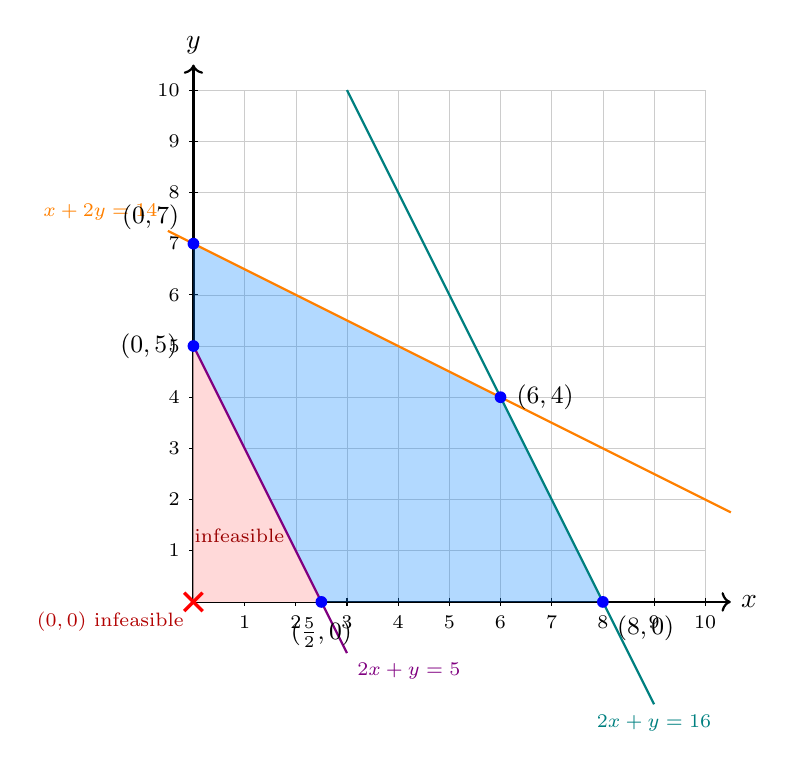
\begin{tikzpicture}[scale=0.65]
    % Grid and axes
    \draw[gray!40, very thin, step=1] (0,0) grid (10,10);
    \draw[->, thick] (0,0) -- (10.5,0) node[right] {$x$};
    \draw[->, thick] (0,0) -- (0,10.5) node[above] {$y$};
    \foreach \x in {1,...,10} \draw (\x,0.08) -- (\x,-0.08) node[below] {\scriptsize \x};
    \foreach \y in {1,...,10} \draw (0.08,\y) -- (-0.08,\y) node[left] {\scriptsize \y};

    % Shade the infeasible "below 2x+y=5" wedge inside the first quadrant
    % lightly, to emphasize that the origin is cut off.
    \fill[red!15] (0,0) -- (2.5,0) -- (0,5) -- cycle;
    \node[red!60!black] at (0.9,1.3) {\scriptsize infeasible};

    % Feasible region
    \fill[blue!50!cyan, opacity=0.3]
        (2.5,0) -- (8,0) -- (6,4) -- (0,7) -- (0,5) -- cycle;

    % Constraint boundaries
    % 2x + y = 5 (purple) - the >= constraint
    \draw[violet, thick] (0,5) -- (3,-1) node[below right] {\scriptsize $2x+y=5$};
    % 2x + y = 16 (teal)
    \draw[teal,   thick] (3,10) -- (9,-2)  node[below] {\scriptsize $2x+y=16$};
    % x + 2y = 14 (orange)
    \draw[orange, thick] (-0.5,7.25) node[above left] {\scriptsize $x+2y=14$} -- (10.5,1.75);

    % Vertices of feasible region
    \node[fill=blue,circle,inner sep=1.5pt,label={below:\small$(\tfrac{5}{2},0)$}]      at (2.5,0) {};
    \node[fill=blue,circle,inner sep=1.5pt,label={below right:\small$(8,0)$}]            at (8,0)   {};
    \node[fill=blue,circle,inner sep=1.5pt,label={right:\small$(6,4)$}]                  at (6,4)   {};
    \node[fill=blue,circle,inner sep=1.5pt,label={above left:\small$(0,7)$}]             at (0,7)   {};
    \node[fill=blue,circle,inner sep=1.5pt,label={left:\small$(0,5)$}]                   at (0,5)   {};

    % Origin: highlight that it is infeasible (draw a small X)
    \draw[red, very thick] (-0.18,-0.18) -- (0.18,0.18);
    \draw[red, very thick] (-0.18, 0.18) -- (0.18,-0.18);
    \node[red!70!black, below left] at (0,0) {\scriptsize $(0,0)$ infeasible};
\end{tikzpicture}
\end{document}
